\documentclass[10pt]{article}
\usepackage{icmlko}

\icmlmeta{IP 파운데이션 월드모델}{250}{교차항은 이름에 산다}{같은 자료 · 같은 열인데 이름을 나눠 쓰느냐로 교차항이 0.18 과 1.01 로 갈린다}

\begin{document}

\twocolumn[
\icmlheader

\begin{abstract}
노트 249는 부호화 변경의 손익이 도메인에 나눠 붙지 않는다는 것을 보였다
(교차항/부분합 $=$ 0.98). 그 노트가 남긴 물음 --- \textbf{축 \emph{추가}도
같은 병인가}. 노트 239--242가 전부 축 추가였으니 답이 절차 전체에 걸린다.
쟀더니 \textbf{아니다}: 도메인 전용 이름을 단 열을 더하면 교차항/부분합이
\textbf{0.27}(다섯 도메인) · \textbf{0.18}(셋)로, 애니는 부분합 $-$0.0251 에
전체 $-$0.0252 로 \textbf{소수 넷째 자리까지 가법}이다. 그러면 무엇이
노트 249와 다른가. 짐작이 하나 있었다 --- 내가 더한 열은 \emph{도메인마다
제 이름}이라 계수를 안 나눠 쓴다. 그 짐작이 검정을 낳는다: \textbf{같은
열에 이름을 하나만 주면 교차항이 살아나야 한다.} 살아났다 ---
\textbf{1.01}. 자료도 같고 열도 같고 오직 이름만 다른데 교차항이 \textbf{5.6
배}다. 이름을 공유한 판에서 애니는 혼자 $-$0.0197 · 남만 $-$0.0322 로
부분합이 $-$0.0519 인데 전체는 $+$0.0002 다 --- \textbf{교차항이 가법 효과를
통째로 지운다.} 그러니 노트 249의 법칙은 ``부호화 대 축 추가''가 아니라
\textbf{``계수를 나눠 쓰느냐''}로 다시 써야 한다. 실용적으로는 좋은 소식이다.
노트 239--242의 축 추가 측정은 전용 이름이었으므로 \textbf{그대로 유효하고},
조심할 곳은 손 축 다섯처럼 \emph{이미 계수를 공유하는} 것을 건드릴 때다.
\end{abstract}
]

\section{축 추가는 가법이다}

노트 249는 손 축 다섯의 부호화를 바꿔 보고 교차항이 부분합만큼 크다는 것을
쟀다(0.98). 남은 물음은 축 \emph{추가}였다. 이 실험실이 노트 239부터 242까지
한 일이 전부 축 추가라, 만약 같은 병이라면 그 측정들을 다시 봐야 한다.

노트 241이 만든 열을 썼다 --- \texttt{target\_breadth} 를 그대로 복사해
\texttt{own\_tb\_<도메인>} 이라는 \emph{제 이름}으로 더하는 것. 도메인에게
그 축의 전용 기울기를 주는 것과 같다.

\begin{center}\small
\begin{tabular}{lrrrrr}
\hline
도메인 & 혼자 & 남만 & 합 & 전체 & 교차항 \\
\hline
웹툰 & $+$0.0110 & $-$0.0007 & $+$0.0103 & $+$0.0067 & $-$0.0036 \\
\textbf{애니} & $-$0.0197 & $-$0.0054 & $\mathbf{-0.0251}$ &
  $\mathbf{-0.0252}$ & $\mathbf{-0.0001}$ \\
모바일 & $-$0.0025 & $+$0.0010 & $-$0.0015 & $-$0.0039 & $-$0.0024 \\
게임 & $+$0.0124 & $-$0.0084 & $+$0.0040 & $+$0.0072 & $+$0.0032 \\
세계애니 & $-$0.0030 & $-$0.0010 & $-$0.0040 & $-$0.0066 & $-$0.0026 \\
\hline
\end{tabular}
\end{center}

$\sum|$교차항$| / \sum|$부분합$| = \mathbf{0.27}$ 이고, 유일하게 유의한
애니($t{=}-2.33$)는 \textbf{0.4\% 만 교차항}이다. 노트 249의 0.98 과 딴판이다.

\section{짐작을 검정으로 바꿨다}

무엇이 다른가. 노트 249는 \emph{있던} 열의 값을 옮겼고 그 열은 아홉 도메인이
계수를 공유한다. 여기서는 \emph{새} 열을 더했는데 그 열은 도메인마다 제
이름이라 계수를 안 나눈다. 그러면 가르는 것은 ``바꾸기 대 더하기''가 아니라
\textbf{계수 공유}일 수 있다.

이 짐작은 값싼 검정을 낳는다. \textbf{똑같은 열을 더하되 이름을 하나만
준다.} 자료도 같고 열도 같고 오직 이름만 다르다.

\begin{figure}[t]
\centering
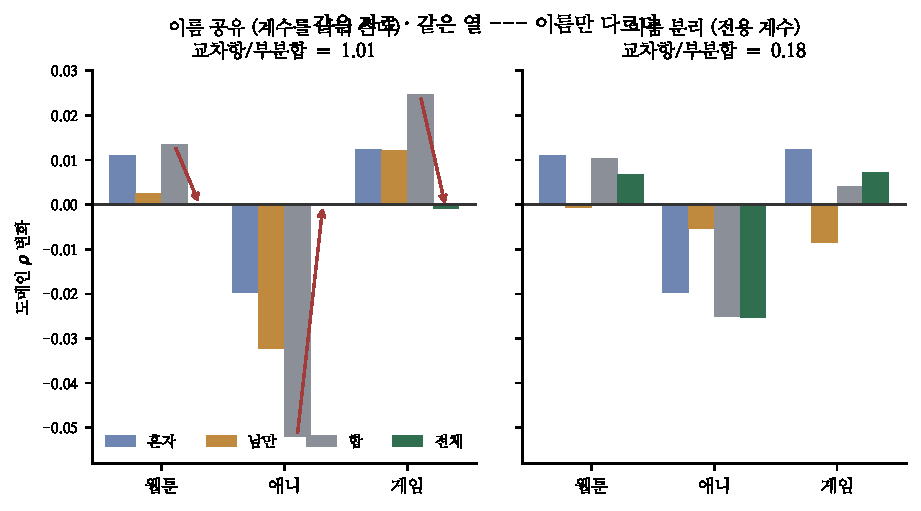
\includegraphics[width=\columnwidth]{figs/names.pdf}
\caption{왼쪽이 이름 공유, 오른쪽이 이름 분리. 빨간 화살표가 교차항이다.}
\end{figure}

\begin{center}\small
\begin{tabular}{lrrrrr}
\hline
\multicolumn{6}{c}{\textbf{이름 공유}} \\
도메인 & 혼자 & 남만 & 합 & 전체 & 교차항 \\
\hline
웹툰 & $+$0.0110 & $+$0.0024 & $+$0.0134 & $-$0.0003 & $-$0.0137 \\
\textbf{애니} & $-$0.0197 & $-$0.0322 & $\mathbf{-0.0519}$ &
  $\mathbf{+0.0002}$ & $\mathbf{+0.0521}$ \\
게임 & $+$0.0124 & $+$0.0122 & $+$0.0246 & $-$0.0008 & $-$0.0254 \\
\hline
\multicolumn{5}{r}{교차항/부분합} & \textbf{1.01} \\
\hline
\end{tabular}
\end{center}

\textbf{살아났다.} 그리고 애니가 극단이다 --- 혼자 $-$0.0197, 남만
$-$0.0322, 부분합 $-$0.0519 인데 \textbf{전체는 $+$0.0002}다. 교차항이
가법 효과를 통째로 지운다. 셋 다 같은 모양이라 판 자체도 $-$0.0006 으로
납작하다.

\begin{center}\small
\begin{tabular}{lr}
\hline
같은 열, 다른 이름 & 교차항/부분합 \\
\hline
이름 분리 (전용 계수) & \textbf{0.18} \\
이름 공유 (계수 나눔) & \textbf{1.01} \\
\hline
\end{tabular}
\end{center}

\textbf{5.6배.} 자료는 한 글자도 안 바뀌었다.

\section{법칙을 다시 쓴다}

\begin{figure}[t]
\centering

\includegraphics[width=\columnwidth]{figs/ratio.pdf}
\caption{네 실험. 빨강 둘이 계수를 나눠 쓰는 경우다.}
\end{figure}

\begin{center}\small
\begin{tabular}{llr}
\hline
무엇을 & 계수 & 교차항/부분합 \\
\hline
축 추가 & 전용 & 0.27 \\
축 추가 & 전용 & 0.18 \\
축 추가 & \textbf{공유} & \textbf{1.01} \\
부호화 변경(노트 249) & \textbf{공유} & \textbf{0.98} \\
\hline
\end{tabular}
\end{center}

노트 249는 법칙을 ``부호화 변경은 나눠 붙일 수 없다''로 적었다. 그것은
사례를 법칙으로 오해한 것이다. 옳은 형태는

\begin{quote}
\textbf{도메인들이 계수를 나눠 쓰는 자리를 건드리면 손익이 짝에 실린다.}
무엇을 바꾸는지(값이냐 열이냐)는 상관없다.
\end{quote}

기전도 이 형태로 읽으면 당연하다. 전용 계수는 A 를 건드려도 B 의 계수가
안 움직인다 --- 남는 결합은 능형 벌점을 통한 간접적인 것뿐이라 작다. 공유
계수는 A 의 값이 바뀌면 \emph{B 가 쓰는 그 계수}가 다시 맞춰지고, B 도
같이 바뀌면 새 계수와 새 값이 동시에 어긋난다.

\section{좋은 소식이다}

실용적 결론이 노트 249보다 훨씬 낫다.

\begin{itemize}
\item 노트 239--242의 축 추가 측정은 \textbf{전용 이름}이었으므로 그대로
유효하다. 다시 안 봐도 된다.
\item 조심할 곳은 \emph{이미} 계수를 공유하는 것 --- \textbf{손 축 다섯}뿐이다.
거기서는 도메인별 A/B 가 무효고(노트 249) 전 도메인 동시 변경으로만 재야
한다.
\item 그리고 새 축을 더할 때 \textbf{이름을 공유할지 나눌지가 측정 가능성
자체를 바꾼다.} 공유하면 도메인별로 못 재게 된다.
\end{itemize}

노트 241이 ``이름을 공유하면 이득이 사라진다''($+$0.0102 $\to$ $+$0.0005)를
쟀을 때는 그것을 \emph{이득}의 이야기로 읽었다. 이제 보면 같은 사실의 다른
얼굴이다 --- \textbf{이름을 공유하면 효과가 짝으로 옮겨 가고, 짝에 실린
효과는 서로 지운다.}

\paragraph{남은 것}
\begin{center}\small
\begin{tabular}{ll}
\hline
갈래 & 왜 \\
\hline
애니 $+$0.0521 & 가법 효과를 정확히 지운다. 우연인가 구조인가 \\
공유를 줄이면 & 손 축 다섯을 전용으로 바꾸면? 노트 241이 $-$0.031 \\
트리 & F18은 계수가 없다. 같은 병인가 \\
웹툰 부호 갈림 & 남이 바꾸면 $+$0.035(노트 249). 아직 안 갈랐다 \\
\hline
\end{tabular}
\end{center}

\paragraph{규약} 측정 전에 \textbf{건드리는 것이 공유 계수인지 본다.}
공유면 도메인별로 재지 말고 전 도메인 동시 변경으로만 재라. 전용이면
도메인별 측정이 유효하다(교차항 0.2 안팎).

\end{document}
